\chapter{ZweiteErfahrung} \label{cha:ZweiteErfahrung}

In diesem Kapitel wird der durch die Projektgruppe implementierte VXI-11-Server vorgestellt und in den einzelnen Abschnitten auf die Teilbereiche Hardware, Software und auf Kommunikationsschnittstellen mit Test- und Messgeräten eingegangen. Die grundlegende Idee des VXI-11-Servers ist die Kommunikation mit Geräten über Ethernet, welche unterschiedliche Kommunikationsstandards nutzen. Hierzu ist eine entsprechende Hardware notwendig, um verschiedenste Kommunikationsstandards anschließen zu können und eine entsprechende softwaretechnische Implementierung. Auf die Realisierung dieser Teilbereiche wird im folgenden eingegangen.

\section{Grundlegende Einführung} 
\cite{lin1973}.

\section{Bildregistrierung} 

\begin{figure}[htb]
 \centering 
 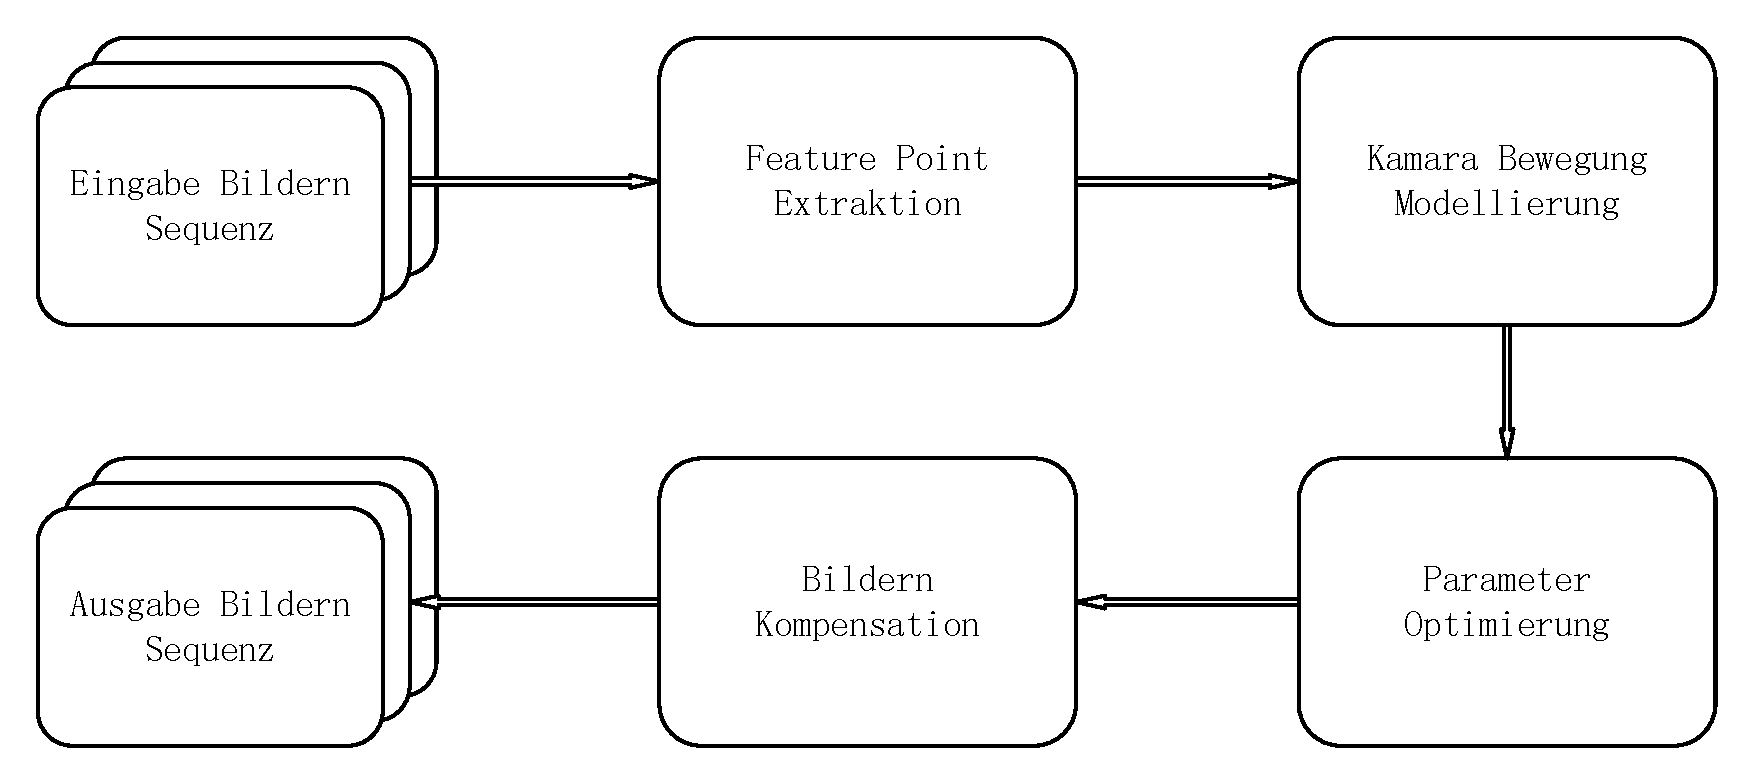
\includegraphics[keepaspectratio,width=0.8\textwidth]{images/0_Image_Registration_Flussdiagramm.pdf}
 \caption{Flussdiagramm der Bildregistrierung}
 \label{fig:Bildregistrierung}
\end{figure}

\subsection{SURF}
Hier wird zuerste die SURF\cite{Surf} Merkmalserkennung eingegangen. SURF Merkmalserkennung arbeitet mit integrierten Bildern. Die Faltung bezieht sich nur auf das vorherige Bild, mit Erhöhung der Größe des Bildkerns können das Heruntertaktung-Verfahren realisiert werden. 

\textbf{Algorithmus:}\\
\\
$\bullet$ \textbf{Aufbau einer hessischen Matrix.}\\
Die Hesse-Matrix stellt den Kern des SURF Algorithmus dar. Zur Vereinfachung der Operation wird die Funktion f (z, y) angenommen, dass die Hesse-Matrix H setzt sich aus Funktionen und partiellen Ableitungen zusammen:

\begin{equation}
   \mathcal{H}(f(x,y)) = \begin{bmatrix}
   \frac{\partial^{2}f}{\partial x^{2}} & \frac{\partial^{2}f}{\partial x \cdot \partial y} \\
   \frac{\partial^{2}f}{\partial x \cdot \partial y} & \frac{\partial^{2}f}{\partial y^{2}} \\   
   \end{bmatrix}
\end{equation}

 Diskriminante der H-Matrix läuft:
 
\begin{equation}
   \det(\mathcal{H}) = \frac{\partial^{2}f}{\partial x^{2}} \cdot \frac{\partial^{2}f}{\partial y^{2}} - (\frac{\partial^{2}f}{\partial x \cdot \partial y})^2  
\end{equation}

Der Wert der Diskriminante ist der Eigenwert der H-Matrix. Durch dessen positiven und negativen wird bestimmt, ob der Punkt ein Extrempunkt ist oder nicht. Im SURF Algorithmus wird das Bildpixel $l(x,y)$ anstelle des Funktionswertes $f(x,y)$ verwendet. Nutzen eine Zweite-Order Gaussian Function als Filter. Die zweiten Partielle Ableitungen können durch Faltung zwischen bestimmten Kernen berechnet werden. Dadurch können die Werte der drei Matrixelemente der H-Matrix auch berechnet werden, nämlich die H-Matrix berechnet:

\begin{equation}
\begin{split}
   &\mathcal{H}(\textbf{x},\sigma) = \begin{bmatrix}
   L_{xx}(\textbf{x},\sigma)\ L_{xy}(\textbf{x},\sigma) \\
   L_{xy}(\textbf{x},\sigma)\ L_{yy}(\textbf{x},\sigma)
   \end{bmatrix} \\   
   &L(\textbf{x},\sigma) = G(\sigma)*I(\textbf{x}) \\  
   &G(\sigma) = \frac{\partial^{2}g(\sigma)}{\partial x^{2}}      
\end{split}
\end{equation}


Hier $L_{xx}(\textbf{x},\sigma)$ bedeutet die Faltung der zweiter Gaussian Ableitung $G(\sigma)$ mit dem Bild I in Punkt $\textbf{x}$(x,y), ähnlich für $L_{xy}(\textbf{x},\sigma)$ und $L_{yy}(\textbf{x},\sigma)$. Auf diese Weise kann der Wert der Determinante für jedes Pixel in dem Bild berechnet werden, und dieser Wert kann verwendet werden, um den Merkmalspunkt zu feststellen.
Zur einfacheren Anwendung schlägt Herbert Bay\cite{Surf} vor, L mit einer Approximation ersetzen. Um den Fehler zwischen dem genauen Wert und der Approximation auszugleichen, kann die H-Matrix-Diskriminante wie folgt ausgedrückt werden:

\begin{equation}
   \det(\mathcal{H}_{Approx}) = D_{xx}D_{yy} - (0.9D_{xy})^2  
\end{equation}
\\
$\bullet$ \textbf{Erstellen Maßstab Raum}\\
Der Maßstabsraum $L(\textbf{x},\sigma)$ des Bildes ist die Darstellung dieses Bildes bei unterschiedlichen Auflösungen(Skalierung). Im Bereich der Computer Vision wird der Maßstabsraum symbolisch als Bildpyramide ausgedrückt, wobei die Eingangsbildfunktion wiederholt mit dem Kern der Gaußschen Funktion gefaltet und wiederholt unterabgetastet wird. Diese Methode wird hauptsächlich für die Implementierung des SIFT Algorithmus verwendet. Jede Bildschicht hängt jedoch von der vorherigen Bildschicht ab, und das Bild muss in der Größe angepasst werden. Daher hat diese Berechnungsmethode eine große Kosten in Berechnung. Im Vergleich dazu ist es in SURF durch die Erhöhung der Größe des Bildkerns. Diese ist ein Unterschied zwischen dem SIFT Algorithmus und dem SURF Algorithmus bei der Verwendung des Pyramidenprinzips.
Der Algorithmus ermöglicht, dass mehrere Bilder des Maßstabsraums gleichzeitig verarbeitet werden, ohne dass das Bild unterabgetastet wird, wodurch die Leistung des Algorithmus verbessert wird. Das linke Bild in Abbildung 4.2 ist eine Pyramidenstruktur, die auf herkömmliche Weise erstellt wird, die Größe des Bildes wird geändert, und die Operation wird die Unterebene  unter Verwendung der Gaußschen Funktion wiederholt glätten. Der Surf Algorithmus auf der rechten Seite in Abbildung 4.2 behält das ursprüngliche Bild unverändert und ändert nur die Filtergröße.

\begin{figure}[htb]
 \centering 
 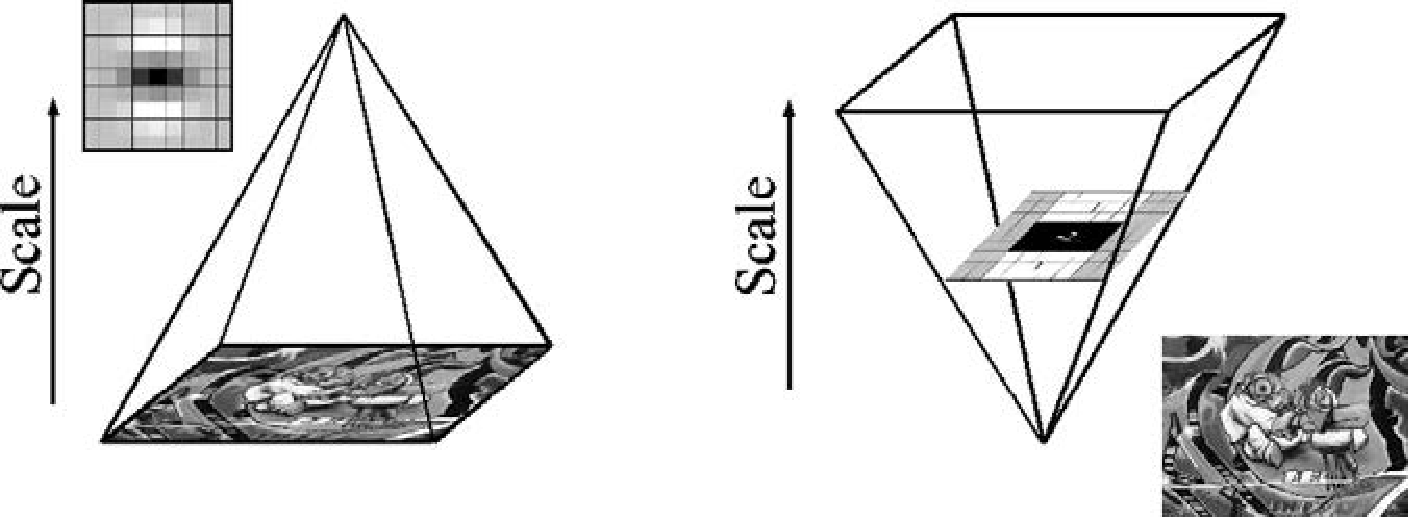
\includegraphics[keepaspectratio,width=0.8\textwidth]{images/4_ZweiteErfahrung/Scale_space.pdf}
 \caption{Scale space}
 \label{fig:Scale space}
\end{figure} 


$\bullet$ \textbf{Präzise Lokalisierung von Feature-Punkten}\\
Vergleichen die Größe jedes Pixel, die von der hessischen Matrix verarbeitet wird, mit die 26 Punkten in seiner drei Dimensionen Raum, wie in Abbildung 4.3 zeight. Wenn es das Maximum oder Minimum dieser 26 Punkte ist, wird es als vorläufiger Merkmalspunkt beibehalten. Das dreidimensionale lineare Interpolationsverfahren wird verwendet, um die Merkmalspunkte des Subpixel-Niveaus zu erhalten, und die Punkte, deren Werte kleiner als ein bestimmter Schwellenwert sind, werden ebenfalls entfernt.

\begin{figure}[htb]
 \centering 
 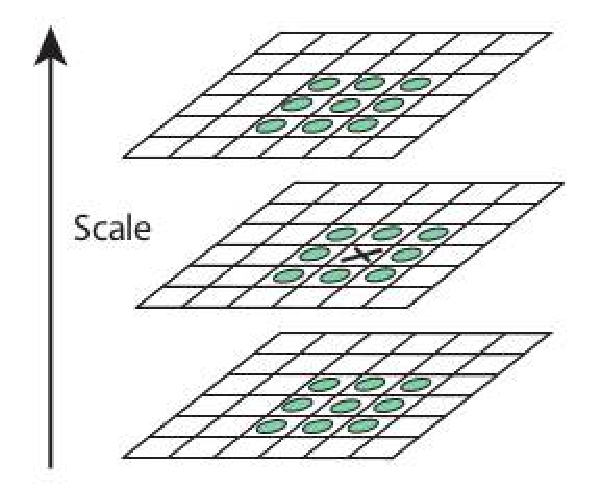
\includegraphics[keepaspectratio,width=0.4\textwidth]{images/4_ZweiteErfahrung/Extreme_Wert_Erkennung.pdf}
 \caption{Extreme Wert Erkennung}
 \label{fig:Extreme Wert Erkennung}
\end{figure} 


$\bullet$ \textbf{Hauptrichtungsermittlung}\\
SIFT wählt die Hauptrichtung des Merkmalspunkts unter Verwendung des Gradientenhistogramms im Merkmalspunktbereich aus. Die Richtung, in der der Bin-Wert des Histogramms der größte und oder 80\% maximale Bin-Wert  überschreitet, wird als Hauptrichtung des Merkmalspunkts genommen. Dagegen beim SURF wird das Gradientenhistogramm nicht statistiken, sondern das Harr-Wavelet-Eigenshcaft im Merkmalspunktbereich wird statistisch analysiert. Das heißt, im Bereich der Merkmalspunkt (zum Beispiel innerhalb eines Kreises mit einem Radius von 6s, wobei s der Maßstab ist, auf dem der Punkt liegt) die Summe der Horizontal-Haar-Wavelet-Merkmale und der Vertikal-Haar-Wavelet-Merkmale aller Punkte im  60-Grad-Sektor($\pi/3$) werden gezählt. Die Größe des Haar Wavelets stellt als 4s, so dass für jeden Sektor einen Wert bekommt. Dann wird 60-Grad-Sektor in einem bestimmten Intervall gedreht, schließlich lassen die Richtung des Sektors mit Maximalwert als Hauptrichtung des Merkmalspunkts nehmen. Ein schematisches Diagramm des Prozesses ist wie folgt in Abbildung 4.4.

\begin{figure}[htb]
 \centering 
 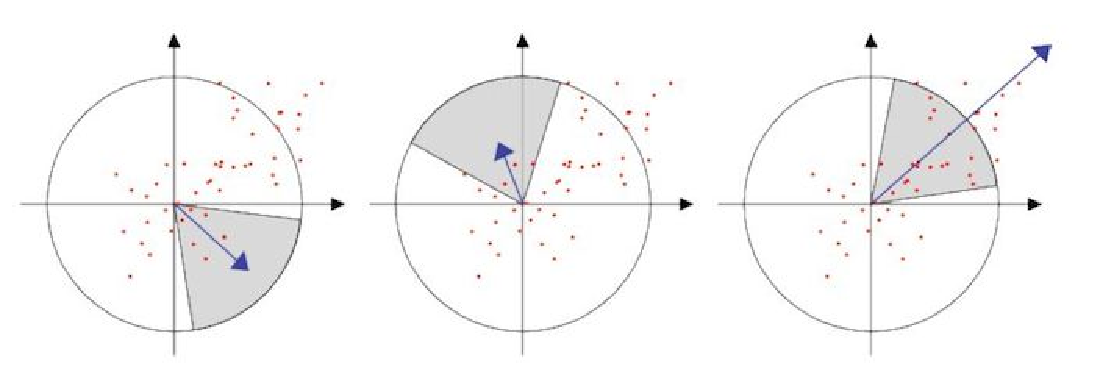
\includegraphics[keepaspectratio,width=0.8\textwidth]{images/4_ZweiteErfahrung/Dominante_Orientierung_Feststellen.pdf}
 \caption{Dominante Orientierung Feststellen}
 \label{fig:Dominante Orientierung Feststellen}
\end{figure} 


$\bullet$ \textbf{Merkmalspunkt Deskriptor Generierung}\\
SURF nehmen eine quadratische Rahmen um den Merkmalspunkt. Die Seite der Rahmen ist 20s (s ist die Skala, bei der der Merkmalspunkt erkannt wird). Die Richtung des Rahmens ist natürlich die Hauptrichtung, die in vorliegened Schritt erfasst wird. Die Rahmen wird dann in 16 Unterbereiche unterteilt, von denen jeder die Haar-Wavelet-Merkmale der horizontalen und vertikalen Richtungen von 25 Pixeln berechnen. Hier die horizontalen und vertikalen Richtungen sind relativ zur Hauptrichtung. Das Haar Wavelet-Merkmal ist die Summe der horizontalen Richtungswerte, die Summe der absoluten Werte in der horizontalen Richtung, die Summe der vertikalen Richtungen und die Summe der absoluten Werte in der vertikalen Richtung. Das schematisches Diagramm in Abbildung 4.5 zeigt dieses Prozesse.

\begin{figure}[htb]
 \centering 
 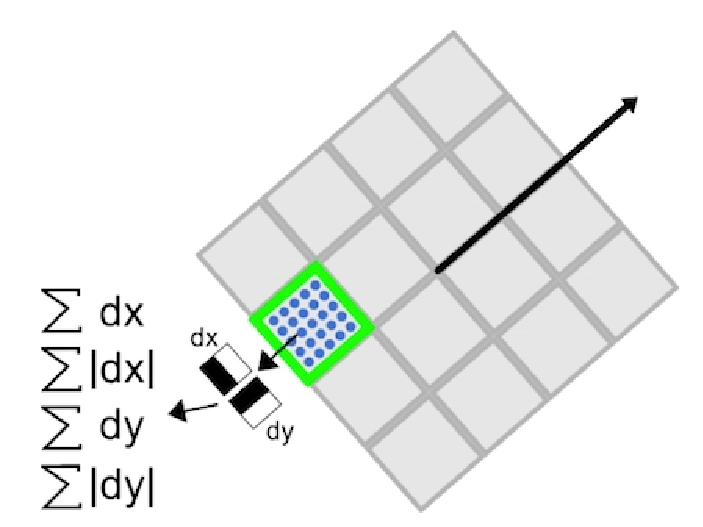
\includegraphics[keepaspectratio,width=0.5\textwidth]{images/4_ZweiteErfahrung/Merkmalspunkt_Deskriptor.pdf}
 \caption{Merkmalspunkt Deskriptor}
 \label{fig:Merkmalspunkt Deskriptor}
\end{figure} 

Auf diese Weise hat jeder kleine Bereich 4 Werte, so dass jeder Merkmalspunkt ein $16*4=64$ dimensionaler Vektor verfügt, der halb so klein wie Sift(128 Dimension) ist, deswegen den Anpassungsprozess beim Merkmalanpassungsprozess stark beschleunigt. Die folgende Abbildung 4.6 zeigt den Merkmalspunkt, den wir durch den SURF-Algorithmus erhalten haben.

\begin{figure}[H]
 \centering 
 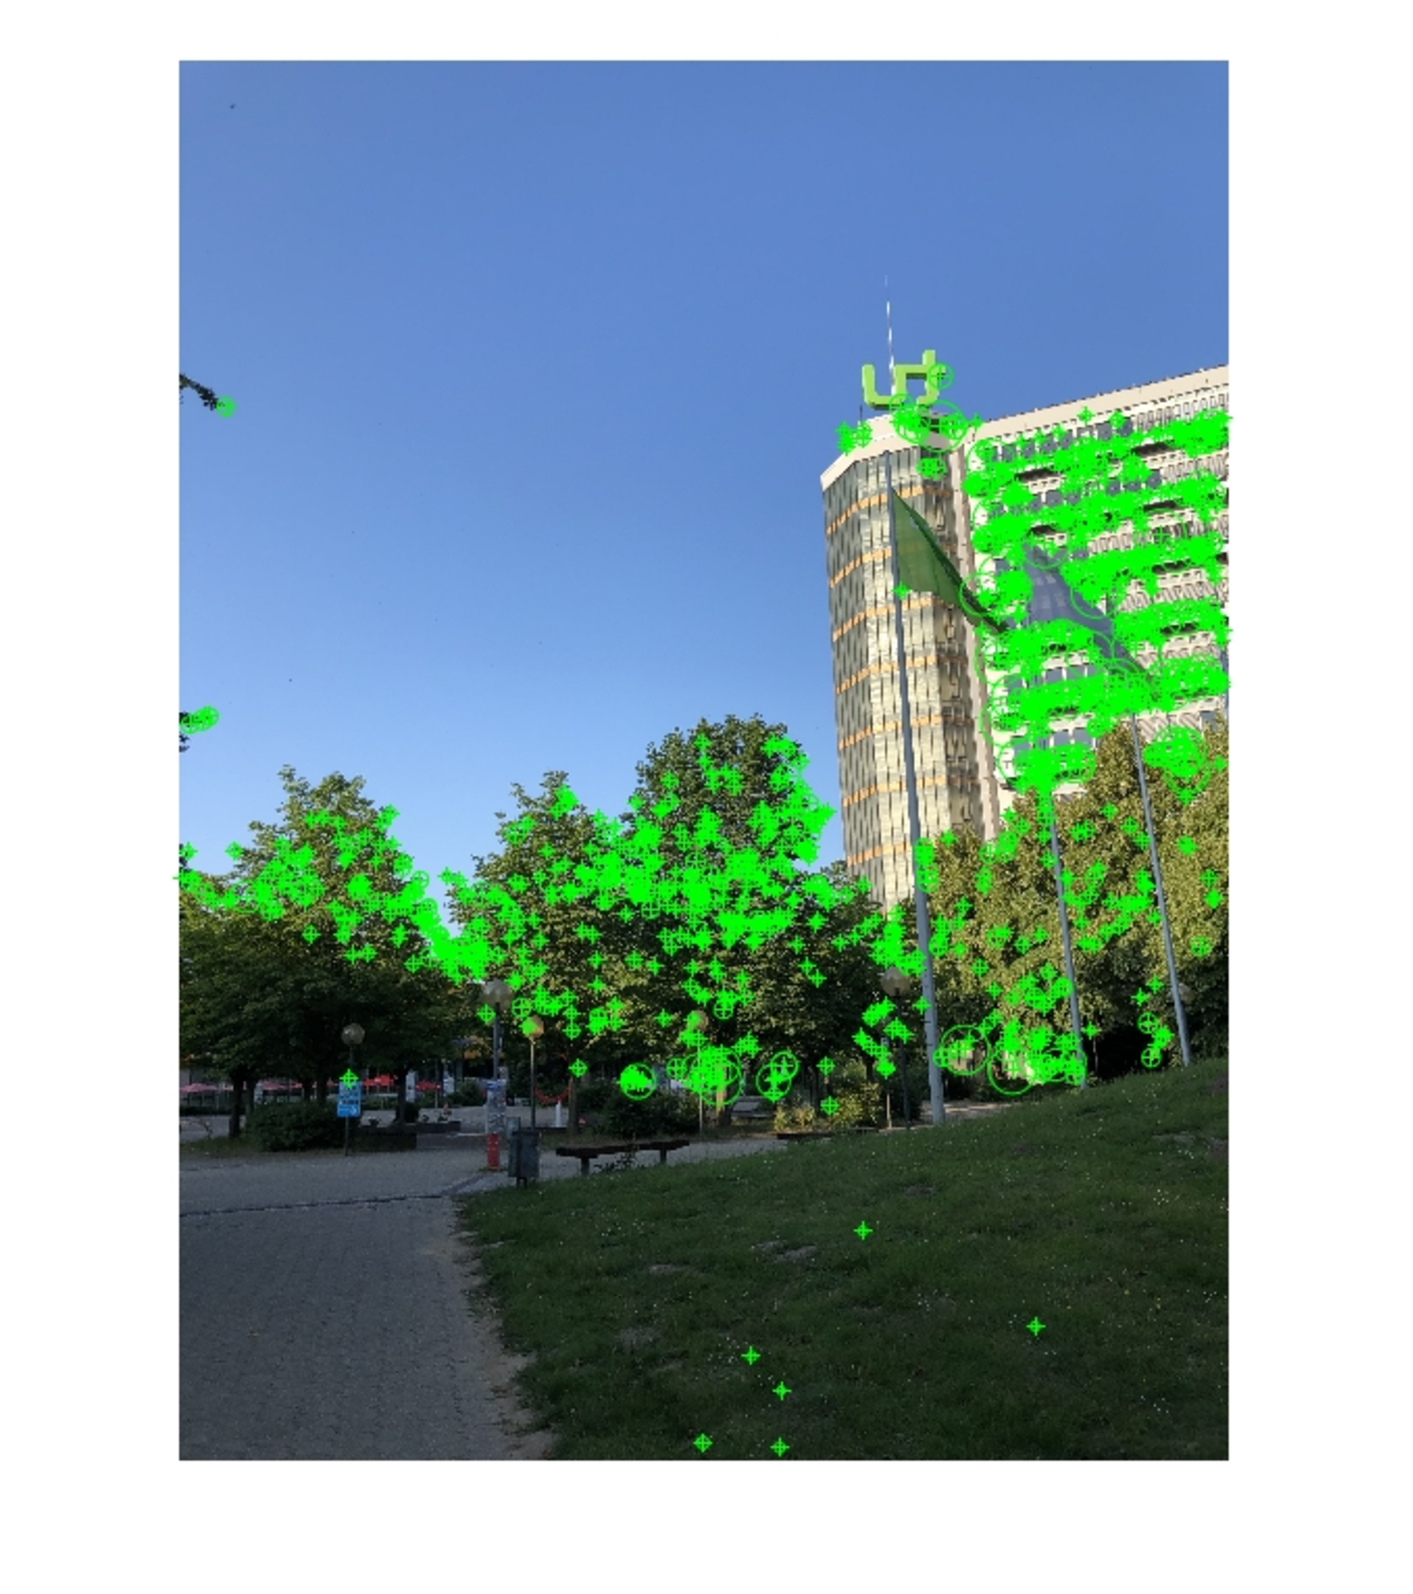
\includegraphics[keepaspectratio,width=0.8\textwidth]{images/4_ZweiteErfahrung/SURF_Detektion.pdf}
 \caption{SURF Merkmal}
 \label{fig:SURF Merkmal}
\end{figure} 


\subsection{RANSAC}

Nach SURF Merkmalserkennung wird die Merkmalspunkte von zwei benachbarten Bildern mit Verfahre z.B. \gls{ncc} übereinstimmt. Abbildung 4.8 zeigt die passende Punkt. Es ist ersichtlich, dass es darin viele fehlerhafte zusammenpassendes Paar gibt. Deswegen wird \gls{ransac} eingeführt.

RANSAC Algorithmus, der von Fischler und Bolles \cite{ransac1} vorgeschlagene im Jahr 1981, ist ein allgemeiner Parameterschätzungsansatz, um den großen Anteil von Ausreißern in den Eingabedaten zu bewältigen. Im Gegensatz zu vielen der üblichen robusten Schätzverfahren wie M-Schätzer und kleinsten Quadraten, die von der Computer Vision Community aus der Statistik-Literatur übernommen wurden, wurde RANSAC aus der Computer-Vision-Community entwickelt. 

Ein einfaches Beispiel ist in der Abbildung 4.7 dargestellt. Das Ziel besteht darin, die am besten geeignete Linie unter einer Menge von Datenpunkten zu finden. Wenn es die einfache Methode der kleinsten Quadrate verwenden ,um diese Linie zu finden, wie auf der linken Seite gezeigt, kann es leider nicht richtig finden, da die Methode der kleinsten Quadrate von alle Datenpunkte beeinflusst wird. Dagegen mit RANSAC kann das Modell nur von der inlierer Punkte berechnet werden und die Ergebnisse wie auf der rechten Seite zeigt. 

\begin{figure}[H]
 \centering 
 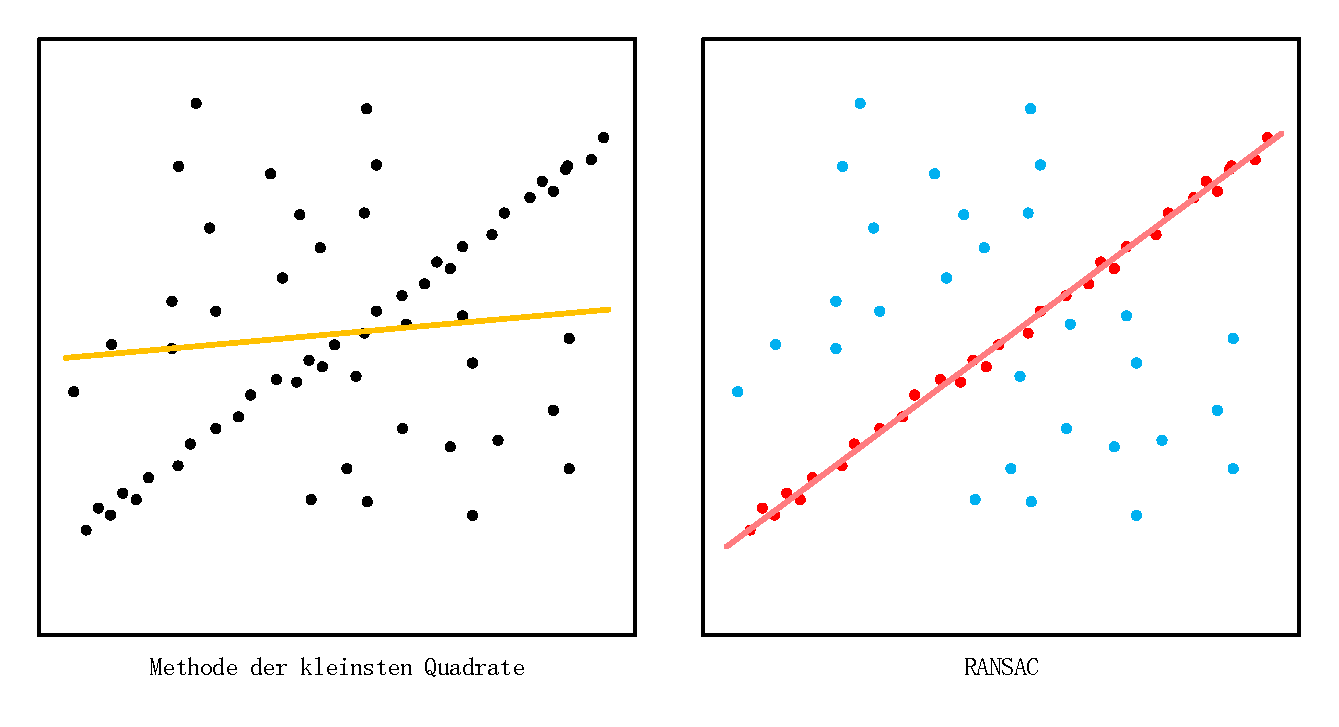
\includegraphics[keepaspectratio,width=1.0\textwidth]{images/4_ZweiteErfahrung/RANSAC/Linien_Detektion.pdf}
 \caption{Linien Detektion}
 \label{fig:Linien Detektion}
\end{figure} 

RANSAC ist ein Wiederholungsprobennahme Verfahren, das  durch die minimalen Anzahl von Beobachtungenpunkten (Datenpunkten) die Kandidatenlösungen generiert. Diese Datebpunkten sind die erforderlich, um die zugrunde liegenden Modellparameter zu schätzen. Darauf haben Fischler und Bolles~\cite{ransac1} hingewiesen, zur Erhalten einer anfängliche Lösung und Beschneidung der Ausreißern RANSAC Verfahren baraucht nicht so viele Daten, sondern verwendet die kleinste mögliche Menge und fährt fort, diese Menge mit eine konsistenten Datenpunkten zu vergrößern.

Der grundlegende Algorithmus ist wie folgt zusammengefasst:

\begin{itemize}
	\item Zufällig wählen die Mindestanzahl der Punkten aus, die erforderlich sind, zum Bestimmen der Modellparameter.
	\item Lösen die Parameter des Modells.
	\item Bestimmen wie viele Punkte aus der Menge aller Punkte mit einer vordefinierten Toleranz $\epsilon$ übereinstimmen
	\item Wenn der Bruchteil der Anzahl von Inlierern über die Gesamtzahl der Punkte in dem Satz einen vordefinierten Schwellenwert $\tau$ überschreitet, schätzen die Modellparameter mit allen identifizierten Inlierern und terminieren wieder.
	\item Ansonsten wiederholen die Schritte 1 bis 4 (maximal N-mal).
\end{itemize}

N bedeutet die Anzahl der Iterationen. Es wird hoch genug gewählt, um die Wahrscheinlichkeit p (normalerweise auf 0,99 gesetzt) sicherzustellen, dass mindestens eine der Gruppen von Stichproben keinen Ausreißer enthält.
Dann die Wahrscheinlichkeit, dass bei N Mal Iterationen mit erforderlich minimalen Anzahl Punkte (hier m annahmen) mindestens ein Ausreißer mit ausgewählt wird, läuft:

\begin{equation}
   1 - p = (1 - u^m)^N
\end{equation}

Hier u stellen die Wahrscheinlichkeit dar, dass jeder ausgewählte Datenpunkt ein Inlier ist. Dagegen $v = 1 - u$ heißt die Wahrscheinlichkeit, dass jeder ausgewählte Datenpunkt ein Ausreißer ist. Durch einige Gleichheitsumwandlung können die Anzahl der Iterationen ausgedrückt werden als:

\begin{equation}
   N = \frac{\log(1 - p)}{\log(1 - (1 - v)^m)}
\end{equation}

In dieser Arbeit werden die Anwendung von RANSAC als folgend Abbildung gezeigt. Abbildung 4.8 zeigt die passende Punkt durch SURF Merkmalserkennung. Es ist ersichtlich, dass es viele fehlerhafte Kombinationen gibt. Durch RANSAC kann dieses Problem lösen und die übereinstimmendenPunkte verfeinern, wie in Abbildung 4.9 zeigt.

\begin{figure}[H]
 \centering 
 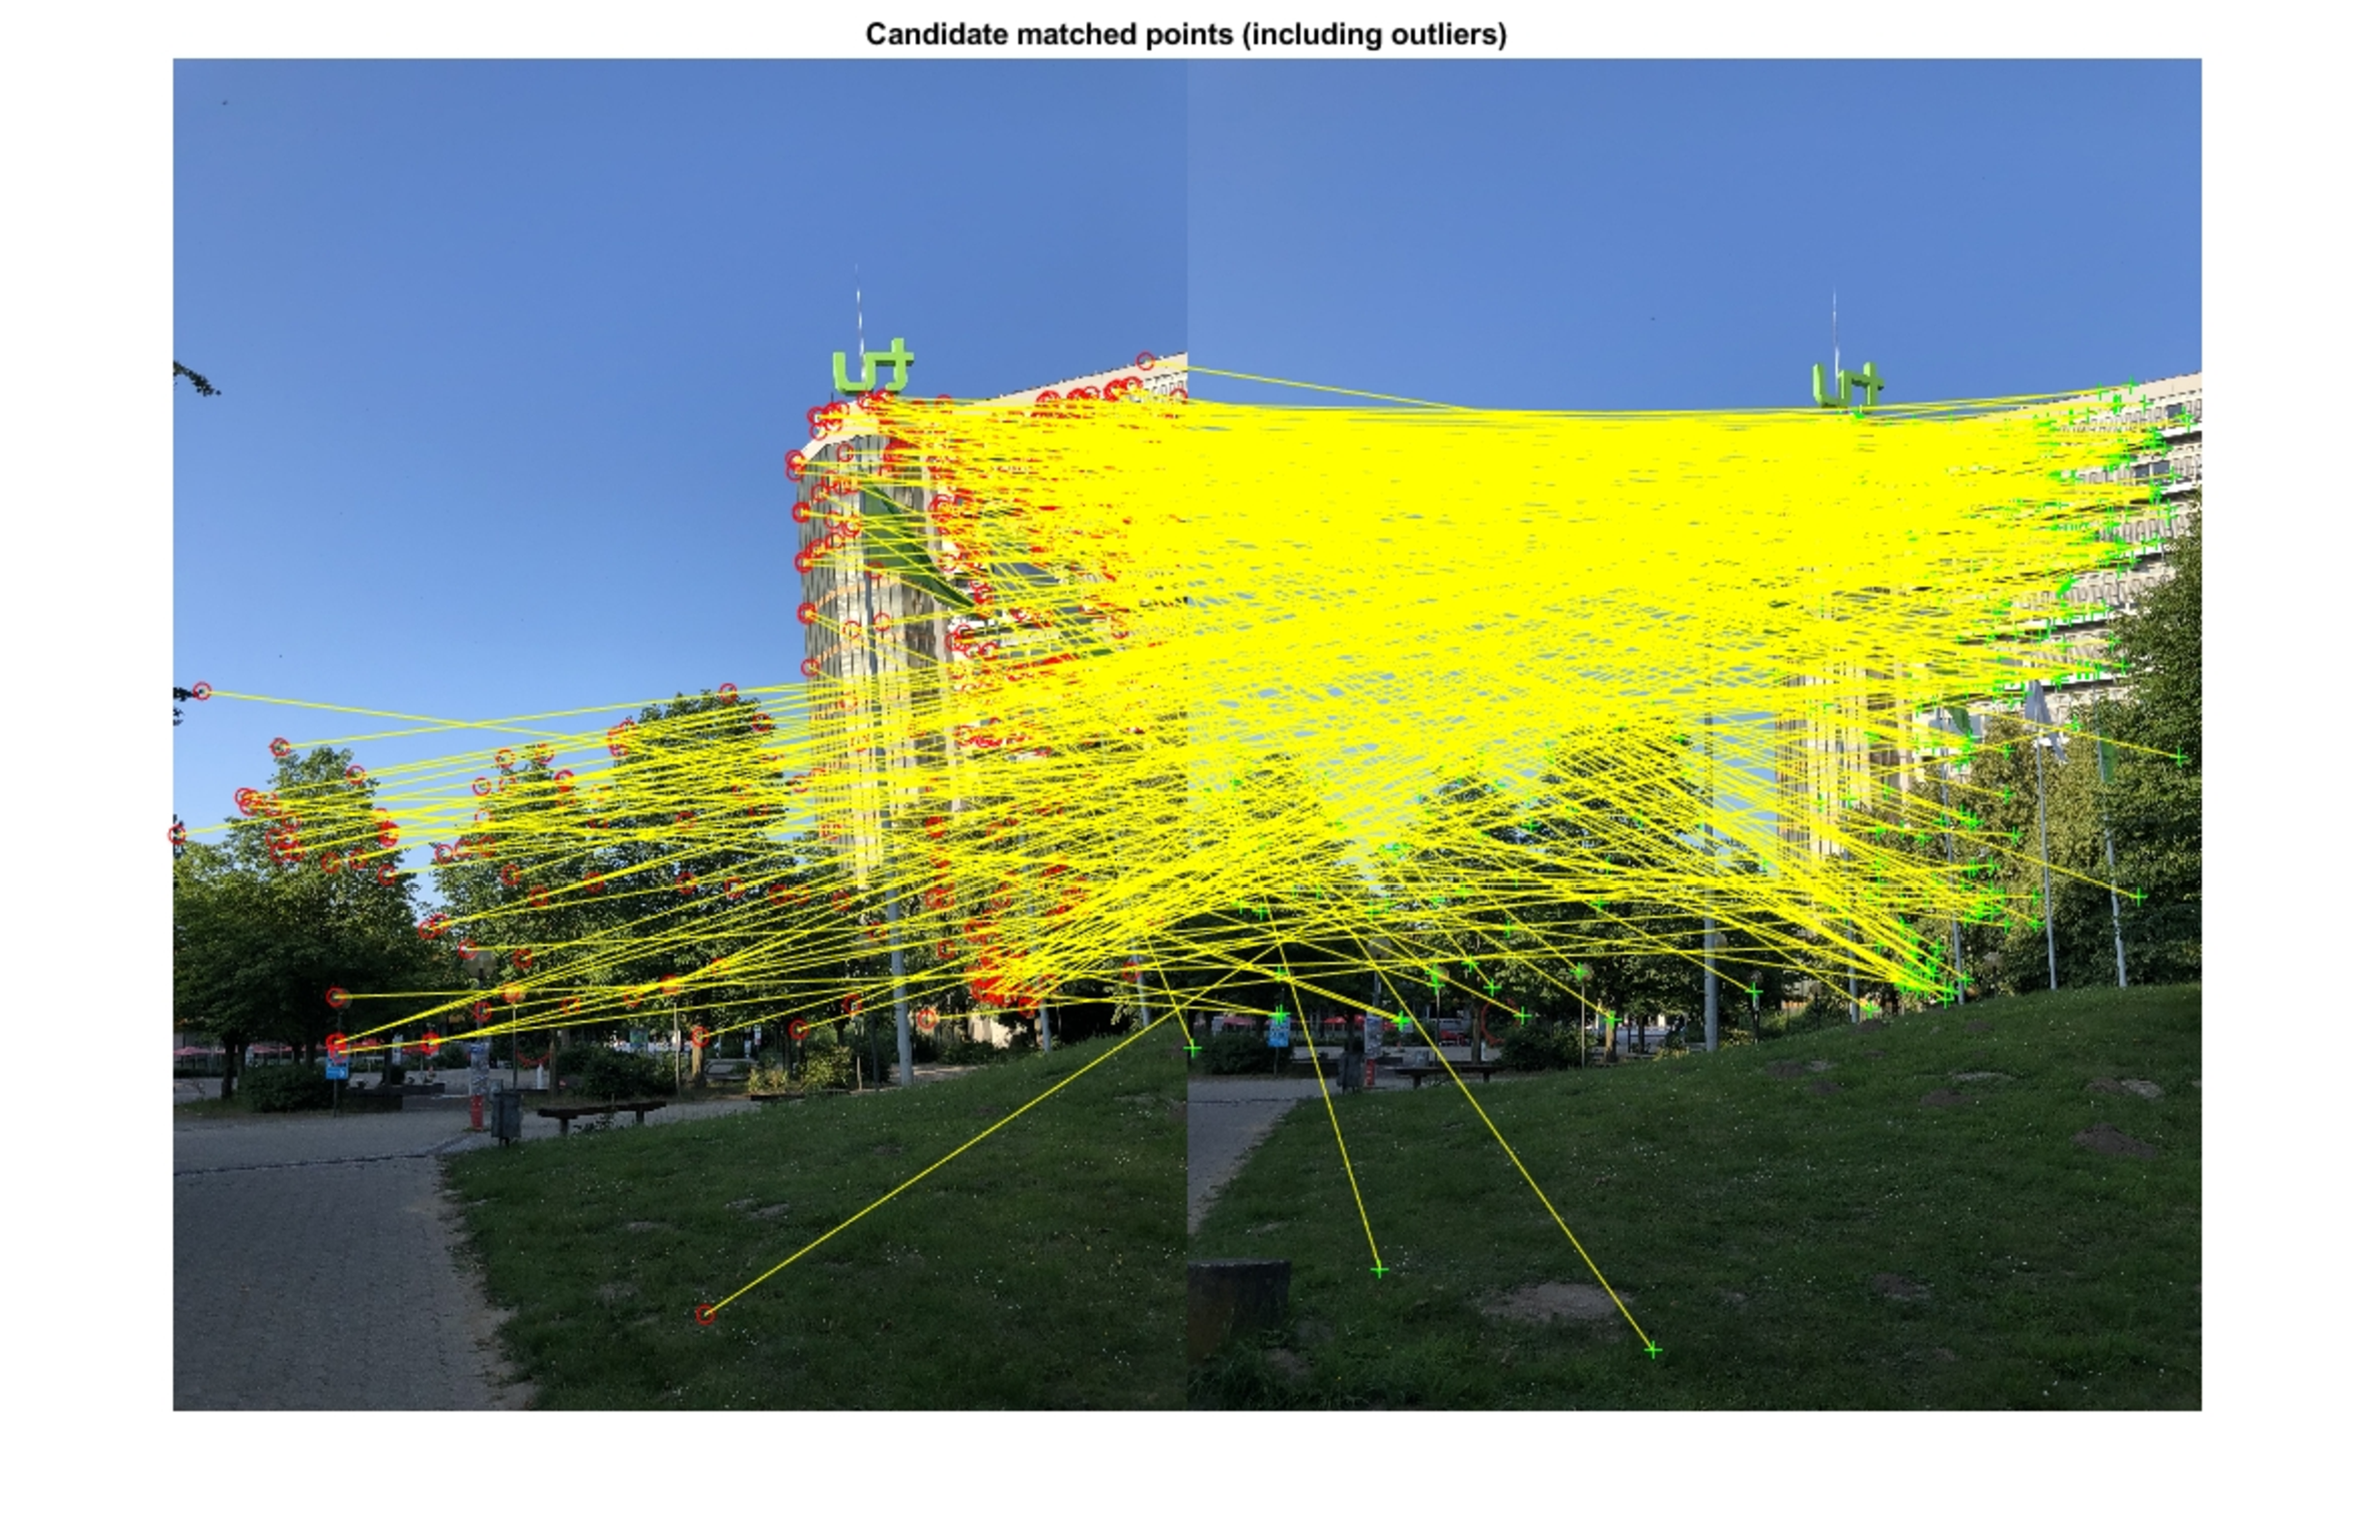
\includegraphics[keepaspectratio,width=0.9\textwidth]{images/4_ZweiteErfahrung/RANSAC/OhneRANSAC.pdf}
 \caption{OhneRANSAC}
 \label{fig:OhneRANSAC}
\end{figure} 

\begin{figure}[H]
 \centering 
 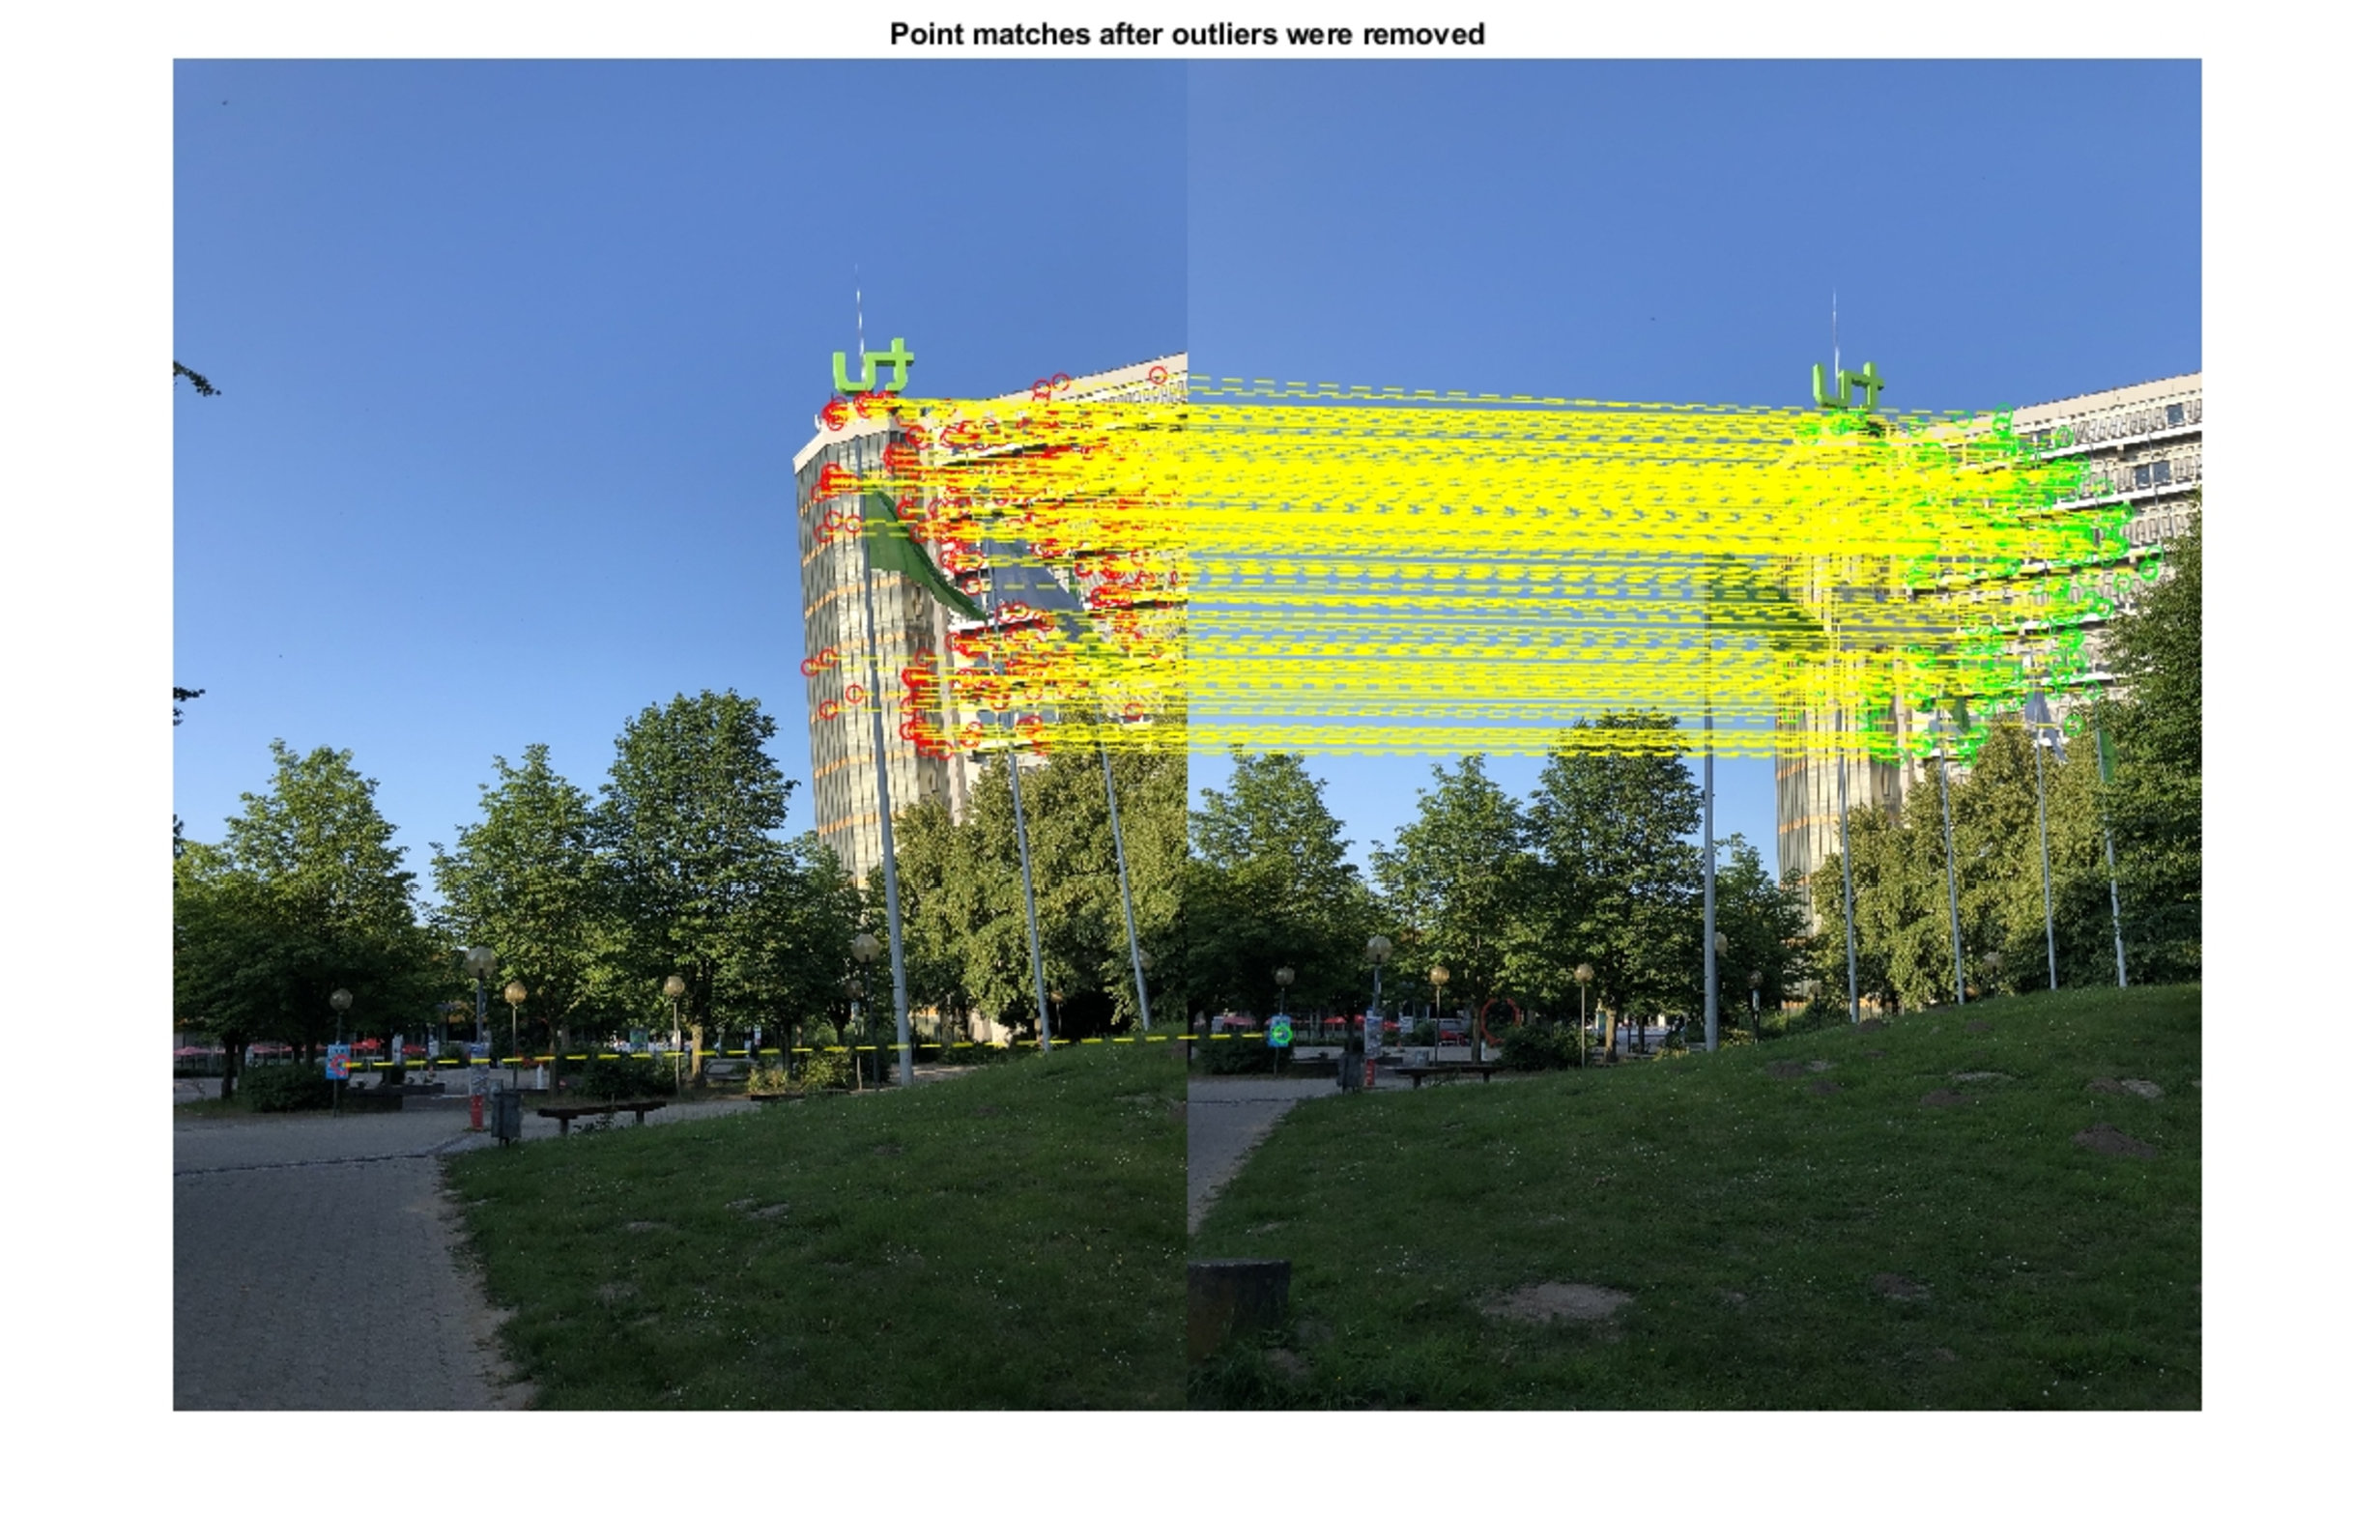
\includegraphics[keepaspectratio,width=0.9\textwidth]{images/4_ZweiteErfahrung/RANSAC/MitRANSAC.pdf}
 \caption{MitRANSAC}
 \label{fig:MitRANSAC}
\end{figure} 


\subsection{Kamerakalibrierung}
Kamara Model

Wie in den ersten beiden Abschnitten vorgestellt,finde  die übereinstimmende Punkte mit Verwenden des SURF in aufeinanderfolgenden Bildern, dann durch RANSAC lassen die Ausreißer verwerfen. Als nächstes soll die Kamera kalibriert werden. In diesem Abschnitt wird zuerst das Kameramodell vorstellt.

\textbf{Kamera Model}

Das Modell der Lochkamera ist in Abbildung 4.10 dargestellt. In dem Modell ist C das optische Zentrum (Fokus), f ist die Kamerabrennweite.

Die vier Koordinatensysteme im Modell sind wie folgt definiert:

\begin{itemize}
	\item 3D Weltkoordinatensystem $W(X,Y,Z)$ \\
	Punktkoordinaten werden durch homogene Koordinaten dargestellt: $\widetilde{X_w}\sim(X_w,Y_w,Z_w,1)^T$
	\item 3D Kamerakoordinatensystem $C(X_c,Y_c,Z_c)$\\
	Punktkoordinaten werden durch homogene Koordinaten dargestellt: $\widetilde{X_c}\sim(X_c,Y_c,Z_c,1)^T$
	\item 2D Bildabbildungs Koordinatensystem $P(x,y)$\\
	Punktkoordinaten werden durch homogene Koordinaten dargestellt: $\widetilde{x}\sim(x,y,1)^T$
	\item 2D Bildpixel Koordinatensystem $I(u,v)$\\
	Punktkoordinaten werden durch homogene Koordinaten dargestellt: $\widetilde{u}\sim(u,v,1)^T$

\end{itemize}


\subsection{Parameter Optimierung}

\section{Differenzbild}


\section{Image Processing} 


\section{QR Pattern Detection} 


